\documentclass[aip, cp, amsmath, amssymb, reprint]{revtex4-2}

\usepackage{graphicx}
\usepackage{dcolumn}
\usepackage{bm}

\usepackage{setspace}
\usepackage{graphicx}% Include figure files
\usepackage{fancyhdr}
\setlength{\parindent}{0in}

% Page Formatting
\pagenumbering{arabic} %\pagenumbering{gobble}
\onehalfspacing %doublespacing
\pagestyle{fancy}
%\usepackage{pdfpages}

% Heading Formatting
\headheight 32pt

% Link Formatting
\usepackage{hyperref}
\hypersetup{
	colorlinks,
	allcolors=black
	%citecolor=black,
	%filecolor=black,
	%linkcolor=black,
	%urlcolor=black
}

\usepackage{mdframed}

\definecolor{commentsColor}{rgb}{0.497495, 0.497587, 0.497464}
\definecolor{keywordsColor}{rgb}{0.541176, 0.168627, 0.886275}
\definecolor{stringColor}{rgb}{0.000000, 0.558215, 0.135316}

% Code Formatting
\usepackage{listings}
\lstset
{ %Formatting for code
	basicstyle=\footnotesize\ttfamily,
	numbers=left,
	%caption={},
	%title={},
	stepnumber=1,
	showstringspaces=false,
	tabsize=1,
	breaklines=true,
	breakatwhitespace=false,
	frame=lines,
	xleftmargin=2em,
	framexleftmargin=1.5em,
	commentstyle=\color{commentsColor}\ttfamily,
  	stringstyle=\color{stringColor}\ttfamily,
	keywordstyle=\color{keywordsColor}\bfseries,
}
\newcommand{\lstprompt}{>\!>\!>}
\newcommand{\numberwithprompt}[1]{\footnotesize\ttfamily\selectfont \lstprompt}


% https://tex.stackexchange.com/questions/340232/how-insert-a-character-at-the-begin-of-every-line-from-a-source-code
\lstdefinestyle{console} {
	basicstyle=\footnotesize\ttfamily,
	numbers=left,
	stepnumber=1,
	showstringspaces=false,
	tabsize=1,
	breaklines=true,
	breakatwhitespace=false,
	frame=single,
	xleftmargin=2em,
	framexleftmargin=2.5em,
	%backgroundcolor=\color{gray!55},
	numberstyle=\numberwithprompt,
	}

% \lstdefinelanguage{psuedocode}{
%   keywords={typeof, new, true, false, catch, function, return, null, catch, switch, var, if, in, while, do, else, case, break},
%   keywordstyle=\color{blue}\bfseries,
%   ndkeywords={class, export, boolean, throw, implements, import, this},
%   ndkeywordstyle=\color{darkgray}\bfseries,
%   identifierstyle=\color{black},
%   sensitive=false,
%   comment=[l]{//},
%   morecomment=[s]{/*}{*/},
%   commentstyle=\color{purple}\ttfamily,
%   stringstyle=\color{red}\ttfamily,
%   morestring=[b]',
%   morestring=[b]"
% }

%\usepackage{algpseudocodex}
%Book Stuff

%\usepackage{algorithm}
%\usepackage[noend]{algpseudocode}
%\makeatletter
%\def\BState{\State\hskip-\ALG@thistlm}
%\makeatother

% Figures & Drawings
\usepackage{graphicx, caption}
\usepackage{animate}
\usepackage{tikz}
\usepackage{float}
\usepackage{pict2e}
\usepackage{subcaption}

% Physics
\usepackage{physics}

% Mathematics
\usepackage{amsmath}
\usepackage{amssymb}
\usepackage{amsthm}
\usepackage{mathtools}
%\usepackage{upgreek} % More Greek letters

% I don't really know what this is but I don't want to break shit
\usepackage{aliascnt}
\newaliascnt{eqfloat}{equation}
\newfloat{eqfloat}{h}{eqflts}
\floatname{eqfloat}{Equation}
\newcommand*{\ORGeqfloat}{}
\let\ORGeqfloat\eqfloat
\def\eqfloat{%
	\let\ORIGINALcaption\caption
	\def\caption{%
		\addtocounter{equation}{-1}%
		\ORIGINALcaption
	}%
	\ORGeqfloat
}
%}

% Bibliography (Citations) Formatting

%\usepackage{cite}
\usepackage{caption}
%\usepackage[backend=bibtex,style=verbose-trad2]{biblatex}
%works really really well, but no MLA format
%\usepackage[backend=biber]{biblatex}
%\bibliographystyle{apsrev4-1}
%\usepackage[backend=biber,style=mla]{biblatex} %Doesn't print all sources for some reason


%\usepackage{graphicx}% Include figure files
\usepackage{dcolumn}% Align table columns on decimal point
\usepackage{bm}% bold math
%\usepackage[mathlines]{lineno}% Enable numbering of text and display math
%\linenumbers\relax % Commence numbering lines

\usepackage[utf8]{inputenc}
\usepackage[T1]{fontenc}
%% Loads a Times-like font. You can also load
%% {newtxtext,newtxtmath}, but not {times}, 
%% {txfonts} nor {mathtpm} as these packages
%% are obsolete and have been known to cause problems.
\usepackage{mathptmx} 


\usepackage{amsthm}
% Tikz Packages
\usepackage{circuitikz}


\tikzset{>=latex} % for LaTeX arrow head
\colorlet{myred}{red!85!black}
\colorlet{mydarkred}{red!55!black}
\colorlet{mylightred}{red!85!black!12}
\colorlet{myfieldred}{mydarkred!5} % for S' background
\colorlet{myredhighlight}{myred!20} % highlights simultaneity in ladder paradox
\colorlet{myblue}{blue!80!black}
\colorlet{mydarkblue}{blue!50!black}
\colorlet{mylightblue}{blue!50!black!30}
\colorlet{mylightblue2}{myblue!10}
\colorlet{mygreen}{green!80!black}
\colorlet{mypurple}{blue!40!red!80!black}
\colorlet{mydarkgreen}{green!50!black}
\colorlet{mydarkpurple}{blue!40!red!50!black}
\colorlet{myorange}{orange!40!yellow!95!black}
\colorlet{mydarkorange}{orange!40!yellow!85!black}
\colorlet{mybrown}{brown!20!orange!90!black}
\colorlet{mydarkbrown}{brown!20!orange!55!black}
\colorlet{mypurplehighlight}{mydarkpurple!20} % highlights simultaneity in ladder paradox
\tikzstyle{world line}=[myblue!40,line width=0.3]
\tikzstyle{world line t}=[mypurple!50!myblue!40,line width=0.3]
\tikzstyle{world line'}=[mydarkred!40,line width=0.3]
\tikzstyle{mysmallarr}=[-{Latex[length=3,width=2]},thin]
\tikzstyle{mydashed}=[dash pattern=on 3 off 3]
\tikzstyle{rod}=[mydarkbrown,draw=mydarkbrown,double=mybrown,double distance=2pt,
                 line width=0.2,line cap=round,shorten >=1pt,shorten <=1pt]
%\tikzstyle{rod'}=[rod,draw=mydarkbrown!80!red!85,double=mybrown!80!red!85]
\tikzstyle{vector}=[->,line width=1,line cap=round]
\tikzstyle{vector'}=[vector,shorten >=1.2]
\tikzstyle{particle}=[mygreen,line width=0.9]
\tikzstyle{photon}=[-{Latex[length=5,width=4]},myorange,line width=0.8,decorate,
                    decoration={snake,amplitude=1.0,segment length=5,post length=5}]

\def\tick#1#2{\draw[thick] (#1) ++ (#2:0.06) --++ (#2-180:0.12)}
\def\tickp#1#2{\draw[thick,mydarkred] (#1) ++ (#2:0.06) --++ (#2-180:0.12)}
\def\Nsamples{100} % number samples in plot
% Custom Symbols 
%{
\newcommand\halmos{\rule{.36em}{2ex}} % Custom QED Symbol
\def\contradict{\tikz[baseline, x=0.22em, y=0.22em, line width=0.032em]\draw (0,2.83)--(2.83,0) (0.71,3.54)--(3.54,0.71) (0,0.71)--(2.83,3.54) (0.71,0)--(3.54,2.83);}
\renewcommand{\qedsymbol}{\halmos}
\renewenvironment{proof}{{\bfseries \textit{Proof} \\}}{\qedsymbol}

\makeatletter
\newcommand{\crossout}[1]{% Crosses out symbol
	\begingroup
	\settowidth{\dimen@}{#1}%
	\setlength{\unitlength}{0.05\dimen@}%
	\settoheight{\dimen@}{#1}%
	\count@=\dimen@
	\divide\count@ by \unitlength
	\begin{picture}(0,0)
		\put(0,0){\line(20,\count@){20}}
		\put(0,\count@){\line(20,-\count@){20}}
	\end{picture}%
	#1%
	\endgroup
}
%}

% Mathematics (General)
\newtheorem{theorem}{Theorem}[section]
\newtheorem{corollary}{Corollary}[theorem]
\newtheorem{lemma}[theorem]{Lemma}

\newcommand{\lemref}[1]{\textit{Lemma \ref{#1}}}
\newcommand{\thmref}[1]{\textbf{Theorem \ref{#1}}}
\newcommand{\colref}[1]{\textit{Corollary \ref{#1}}}

\newcommand{\num}[3]{${#1}\pm{#2} \ \text{{#3}}$}

% Physics (Quantum Mechanics)
%\newcommand{\norm}[#1]{\lVert {#1} \rVert}
%\newcommand{\ket}[1]{\vert{#1}\rangle}
%\newcommand{\bra}[1]{\langle{#1}\vert}
%\newcommand{\braket}[2]{\langle {#1} \vert {#2} \rangle}
\newcommand{\expectation}[1]{\langle{#1}\rangle}

% Physics (Electrodynamics)
\newcommand{\del}{\overline{\nabla}}
\usetikzlibrary{arrows}
%Script r (scalar)
\newcommand{\rc}{%
\resizebox{!}{1.25ex}{%
    \begin{tikzpicture}[>=round cap]
        \clip (0.09em,-0.05ex) rectangle (0.61em,0.81ex);
        \draw [line width=.11ex, <->, rounded corners=0.13ex] (0.1em,0.1ex) .. controls (0.24em,0.4ex) .. (0.35em,0.8ex) .. controls (0.29em,0.725ex) .. (0.25em,0.6ex) .. controls (0.7em,0.8ex) and (0.08em,-0.4ex) .. (0.55em,0.25ex);
    \end{tikzpicture}%
}%
}

%Script r (vector)
\newcommand{\brc}{%
\resizebox{!}{1.3ex}{%
    \begin{tikzpicture}[>=round cap]
        \clip (0.085em,-0.1ex) rectangle (0.61em,0.875ex);
        \draw [line width=.2ex, <->, rounded corners=0.13ex] (0.1em,0.1ex) .. controls (0.24em,0.4ex) .. (0.35em,0.8ex) .. controls (0.29em,0.725ex) .. (0.25em,0.6ex) .. controls (0.7em,0.8ex) and (0.08em,-0.4ex) .. (0.55em,0.25ex);
    \end{tikzpicture}%
}%
}

%Script r with a hat (unit vector)
\newcommand{\hrc}{\hat{\brc}}


% Document (General)
\newcommand{\figref}[1]{Fig. \ref{#1}}
\newcommand{\source}[1]{\caption*{Source: {#1}} }
\newcommand{\graphdata}[1]{\caption*{Fit Parameters: {#1}}}
%\newenvironment{\drawpicture}[1][]{\resizebox{<horizontal size>}{<vertical size>}{ \begin{tikzpicture}}{\end{tikzpicture}}}



% ========================================= %
% LaTeX Template by Aditya K. Rao
% Contact at adi.rao@mail.utoronto.ca

% Change for each document [!!!]
\newcommand\course{PHY385}	% Course Code [!!!]
\newcommand\doctitle{Investigation Into The Effect of Polarizors and Waveplates on a Helium-Neon Laser} % Report Title [!!!]
\newcommand\firstauthorname{Aditya K. Rao}
\newcommand\firstauthorstdnum{Student Number: 1008307761}
\newcommand\firstauthoremail{adi.rao@mail.utoronto.ca}
%\newcommand\secondauthorname{Author Two}
%\newcommand\secondauthorstdnum{Student Number: 0000000000}
%\newcommand\secondauthoremail{report.author@mail.utoronto.ca}
\newcommand\advname{Boris Braverman } % Advisor Name [!!!]  
\newcommand\taname{Michael Sloan } % Advisor Name [!!!]   
\newcommand{\location}{MP222} % Location [!!!]
% ========================================= %
 
% ============== EQUIPMENT ================ %

\newcommand{\oscope}{\texttt{DSOX1202G}\,}
\newcommand{\pdiode}{\texttt{DET36A2}\,}
\newcommand{\hene}{\texttt{HNLS008L}\,}

% ========================================= %

%\pagenumbering{gobble}
\usepackage{listings}

\renewcommand\lstlistingname{Code Reference}
\renewcommand\lstlistlistingname{Code Reference}
\usepackage{tikz}
\usetikzlibrary{patterns}

\usepackage{circuitikz}

%\addbibresource{references.bib}
\usepackage{lipsum}
\usetikzlibrary{calc}

\begin{document}
\onecolumngrid
\pagenumbering{arabic}
\title{\doctitle}
\author{\firstauthorname}
\email{\firstauthoremail}
\thanks{\firstauthorstdnum}
%\email{report.author@mail.utoronto.ca}
%\thanks{Student Number: 0000000000}
\affiliation{
University of Toronto \\
\location, 60 St. George Street, Toronto, Ontario M5S 1A7, Canada.% Force line breaks with \\ if necessary
}

\date{\today} %Put in date of submission [!!!]

\preprint{APS/123-QED}
\begin{abstract}
    ABSTRACT
\end{abstract}
    \maketitle
    \tableofcontents 

    \lhead{\firstauthorname\vspace{0.1cm}}
    \chead{\textbf{\course} \\ \doctitle}
    \rhead{\textbf{Prof:} \advname \\ \textbf{Loc:} \location}
    \nocite{*}

    \newpage
    \twocolumngrid
    \section{Introduction}
        Electromagnetic waves are modeled as transverse plane waves that oscillate in the direction perpendicular to their propagation. The electric field of these waves can be described by \eqref{eqn:electric_field}.
    
        \begin{equation} \label{eqn:electric_field}
            \vec{E}_0 = E_i\hat{i} + E_J\hat{j}
        \end{equation}

        One properties of such waves is their ability to become `polarized'. This annihlates all other oscillations apart from a single plane. This can be achieved by passing the wave through a polarizer. The intensity of the light that passes through the polarizer is given by \eqref{eqn:malus}. 

        \begin{equation} \label{eqn:malus}
            I = I_0 \cos^2(\theta)
        \end{equation}

        In this experiment, the power is recorded as opposed to the intensity. However, because the power is proportional to the intensity, the same equation can be used. The power of an Electromagnetic wave is directly proportional to the product of its electric field and its complex conjugate. This is given by \eqref{eqn:power}. 

        \begin{equation} \label{eqn:power}
            P \propto |E_0|^2
        \end{equation}

        Waveplates are another common optical element which, instead of restricting the oscillations of the electric field, shift the phase of the wave. This is done by changing the refractive index of the material.
        
        \begin{equation} \label{eqn:generalized-polarizer}
            \hat{\Pi}_{\theta} = \begin{bmatrix} \cos^2(\theta) & \sin(\theta)\cos(\theta) \\ \sin(\theta)\cos(\theta) & \sin^2(\theta)\end{bmatrix}
        \end{equation}

        \begin{equation} \label{eqn:jones-mat}
            \hat{J} = \chi\hat{\Pi}_{0'} + \zeta\hat{\Pi}_{1'}
        \end{equation}

        Here, two different types of waveplate will be investigated: quarter and half waveplates. The quarter waveplate shifts the phase of the wave by $\pi/2$ radians. The half waveplate shifts the phase of the wave by $\pi$ radians. The resultant effect on the power should be that the power is unchanged for the half wave plate and that the power is reduced for the quarter waveplate due to destructive and constructive interference of the $E_x$ and $E_y$ components.

        The jones matrix for a waveplate is given by \eqref{eqn:jones-mat}. Here, $\chi$ and $\zeta$ are the complex amplitudes of the electric field. For the quarter waveplate, the Jones matrix is given by \eqref{eqn:quarter-waveplate}. For the half waveplate, the Jones matrix is given by \eqref{eqn:half-waveplate}.
        \begin{minipage}{\linewidth}
        \centering
        \begin{minipage}{0.55\linewidth}
            \begin{equation} \label{eqn:quarter-waveplate}
                \hat{J}_{QWP} = \begin{bmatrix} 1 & 0 \\ 0 & \exp\left\{\frac{i\pi}{2}\right\}\end{bmatrix}
            \end{equation}
        \end{minipage}
        \begin{minipage}{0.44\linewidth}
            \begin{equation} \label{eqn:half-waveplate}
                \hat{J}_{HWP} = \begin{bmatrix} 1 & 0 \\ 0 & -1\end{bmatrix}
            \end{equation}
        \end{minipage}
        \end{minipage}
        % \begin{equation} \label{eqn:quarter-waveplate}
        %     \hat{J}_{QWP} = \begin{bmatrix} 1 & 0 \\ 0 & e^{i\pi/2}\end{bmatrix}
        % \end{equation}

        % \begin{equation} \label{eqn:half-waveplate}
        %     \hat{J}_{HWP} = \begin{bmatrix} 1 & 0 \\ 0 & -1\end{bmatrix}
        % \end{equation}

    \section{Methodology}
        Two experiments were conducted in order to test and verify the effects of polarizrs and waveplates on a Helium-Neon (HeNe) laser with an additional third being planned. The experimental setup for each is shwon in Figures \ref{fig:exp1-setup} and \ref{fig:exp2-setup} respectively. 
        
        For each experiment, a \texttt{PDA015C2} photodiode was used to measure the intensity of the light. The photodiode was connected to a \texttt{DSO } oscilloscope which was used to measure the voltage output from the optical setup. The HeNe laser was the first component attached to the optical breadboard. All other components were then roughly placed in position (not clamped) after which fine \& coarse adjustments were made to align the beam path. 

        To reduce ambient light a shroud was put over the photodiode. The resultent baseline voltage dropped from ~2V to $\approx 240 \pm 10 \,\text{mV}$.

        \subsection{Polarizers}
            The second polarizer was removed from the post holder. The polarizer's angle was then adjusted such that the outputed power delivered to the photodiode was below its saturation voltage. This maximum power output was recorded at $V=5.00\,V$. The angle of the polarizer was recorded as $157.69^\circ \pm 0.01^\circ$. 
            
            \begin{figure}[H]
                \centering
                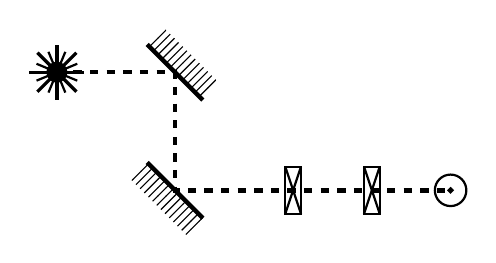
\begin{tikzpicture}
    \coordinate (L) at (0,0);
    \coordinate (M1) at (1.5,0);
    \coordinate (M2) at (1.5,-1.5);
    \coordinate (P1) at (3,-1.5);
    \coordinate (P2) at (4,-1.5);
    \coordinate (D) at (5,-1.5);

    % Laser Symbol
    \begin{scope}[scale=0.7]
        \draw[ultra thick, fill = black] (0,0) circle (0.15);
        \draw[rotate=0, very thick] (-0.5,0) -- (0.5,0);
        \draw[rotate=90, very thick] (-0.5,0) -- (0.5,0);
        \draw[rotate=45, very thick] (-0.5,0) -- (0.5,0);
        \draw[rotate=135, very thick] (-0.5,0) -- (0.5,0);

        \draw[rotate=22.5, thick] (-0.4,0) -- (0.4,0);
        \draw[rotate=67.5, thick] (-0.4,0) -- (0.4,0);
        \draw[rotate=112.5, thick] (-0.4,0) -- (0.4,0);
        \draw[rotate=157.5, thick] (-0.4,0) -- (0.4,0);
    \end{scope}


    % Mirror #1
    \begin{scope}[shift={(M1)}, rotate=-45]
        \draw[ultra thick] (-0.5,0) -- (0.5,0);
        \fill[pattern=north east lines] (-0.5,0) rectangle (0.5,0.30);
        %\coordinate (M1) at (0,-0.15);
    \end{scope}

    % Mirror #2
    \begin{scope}[shift={(M2)}, rotate=135]
        \draw[ultra thick] (-0.5,0) -- (0.5,0);
        \fill[pattern=north east lines] (-0.5,0) rectangle (0.5,0.30);
        %\coordinate (M2) at (0,-0.15);
    \end{scope}

    % Polarizer #1
    \begin{scope}[shift={(P1)}, scale=0.5]
        \draw[thick] (-0.2,0.6) rectangle (0.2,-0.6);
        \draw[thick] (-0.2,0.6) -- (0.2,-0.6);
        \draw[thick] (0.2,0.6) -- (-0.2,-0.6);
        %\coordinate (P1) at (0,0);
    \end{scope}

    % Polarizer #2
    \begin{scope}[shift={(P2)}, scale=0.5]
        \draw[thick] (-0.2,0.6) rectangle (0.2,-0.6);
        \draw[thick] (-0.2,0.6) -- (0.2,-0.6);
        \draw[thick] (0.2,0.6) -- (-0.2,-0.6);
        %\coordinate (P2) at (0,0);
    \end{scope}

    % Detector
    \begin{scope}[shift={(D)}, scale=0.5]
        \draw[thick] (0,0) circle (0.4);
        \draw[thick, fill=black] (0,0) circle (0.05);
        %\coordinate (D) at (0,0);
    \end{scope}

    % Laser Path
    \draw[ultra thick, dashed] (L) -- (M1) -- (M2) -- (P1) -- (P2) -- (D);
\end{tikzpicture}
                \caption{Experimental Setup for Experiment 1}
                \label{fig:exp1-setup}
            \end{figure}
            
            This was kept the same for subsequent measurments. The second polarizer was then varied in angle from $0^\circ$ to $270^\circ$ in increments of $10^\circ$. The voltage output from the photodiode was recorded for each angle.

            To reduce ambient light a shroud was put over the photodiode. The resultent baseline voltage dropped from ~2V to $\approx 240 \pm 10 \,\text{mV}$.

            Upon adding the second polarizer, massive fluctuations in the output voltage were observed (on the order of at least $0.5\,V$, but proportional to the output voltage). This was likely due to an issue with the battery of the photodiode. However, upon replacing the battery, no change in the output was observed. Therefore, the issue was likely within the output of the HeNe laser. The is documented furhter later in the report. In order to mitigate this abnormality, the output voltage was recorded at specific time intervals where the output voltage was semi-stable.

        \subsection{Waveplates}
            The experimental setup in Fig. \ref{fig:exp1-setup} was modified to place a waveplate between the two polarizers. In the first part of the experiment, the effect of a quarter waveplate was tested. The waveplate was placed at an angle of $0^\circ$ with respect to the horizontal. The second polarizer was then varied in angle from $0^\circ$ to $220^\circ$ i\,\text{V}n increments of $20^\circ$. The voltage output from the photodiode was recorded for each angle.

            \begin{figure}[H]
                \centering
                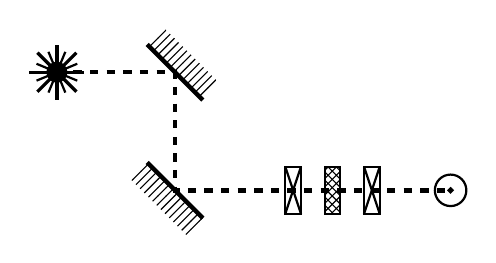
\begin{tikzpicture}
    \coordinate (L) at (0,0);
    \coordinate (M1) at (1.5,0);
    \coordinate (M2) at (1.5,-1.5);
    \coordinate (P1) at (3,-1.5);
    \coordinate (P2) at (4,-1.5);
    \coordinate (W) at (3.5,-1.5);
    \coordinate (D) at (5,-1.5);

    % Laser Symbol
    \begin{scope}[scale=0.7]
        \draw[ultra thick, fill = black] (0,0) circle (0.15);
        \draw[rotate=0, very thick] (-0.5,0) -- (0.5,0);
        \draw[rotate=90, very thick] (-0.5,0) -- (0.5,0);
        \draw[rotate=45, very thick] (-0.5,0) -- (0.5,0);
        \draw[rotate=135, very thick] (-0.5,0) -- (0.5,0);

        \draw[rotate=22.5, thick] (-0.4,0) -- (0.4,0);
        \draw[rotate=67.5, thick] (-0.4,0) -- (0.4,0);
        \draw[rotate=112.5, thick] (-0.4,0) -- (0.4,0);
        \draw[rotate=157.5, thick] (-0.4,0) -- (0.4,0);
    \end{scope}

    % Mirror #1
    \begin{scope}[shift={(M1)}, rotate=-45]
        \draw[ultra thick] (-0.5,0) -- (0.5,0);
        \fill[pattern=north east lines] (-0.5,0) rectangle (0.5,0.30);
    \end{scope}

    % Mirror #2
    \begin{scope}[shift={(M2)}, rotate=135]
        \draw[ultra thick] (-0.5,0) -- (0.5,0);
        \fill[pattern=north east lines] (-0.5,0) rectangle (0.5,0.30);
    \end{scope}

    % Polarizer #1
    \begin{scope}[shift={(P1)}, scale=0.5]
        \draw[thick] (-0.2,0.6) rectangle (0.2,-0.6);
        \draw[thick] (-0.2,0.6) -- (0.2,-0.6);
        \draw[thick] (0.2,0.6) -- (-0.2,-0.6);
    \end{scope}

    % Polarizer #2
    \begin{scope}[shift={(P2)}, scale=0.5]
        \draw[thick] (-0.2,0.6) rectangle (0.2,-0.6);
        \draw[thick] (-0.2,0.6) -- (0.2,-0.6);
        \draw[thick] (0.2,0.6) -- (-0.2,-0.6);
    \end{scope}

    % Wave Plate
    \begin{scope}[shift={(3.5,-1.5)}, scale=0.5]
        \draw[thick, pattern=crosshatch] (-0.2,0.6) rectangle (0.2,-0.6);
    \end{scope}

    % Detector
    \begin{scope}[shift={(D)}, scale=0.5]
        \draw[thick] (0,0) circle (0.4);
        \draw[thick, fill=black] (0,0) circle (0.05);
    \end{scope}

    % Beam Path
    \draw[ultra thick, dashed] (L) -- (M1) -- (M2) -- (P1)-- (W) -- (P2) -- (D);
\end{tikzpicture}
                \caption{Experimental Setup for Experiment 2}
                \label{fig:exp2-setup}
            \end{figure}

            This was then followed by a similar experiment with a half waveplate. The waveplate was placed at an angle of $0^\circ$ with respect to the horizontal. The second polarizer was then varied in angle from $0^\circ$ to $220^\circ$ in increments of $20^\circ$. The voltage output from the photodiode was recorded for each angle.

        \subsection{Dielectrics}
            Due to time constraints, this experiment was not completed in full. The proposed setup is shown in Fig. \ref{fig:exp3-setup}. The setup was to be similar to the previous two experiments, with the addition of a dielectric material between the two polarizers. The dielectric material was to be placed at an angle of $0^\circ$ with respect to the horizontal. The second polarizer was then varied in angle from $0^\circ$ to $220^\circ$ in increments of $20^\circ$. The voltage output from the photodiode was to be recorded for each angle.

            \begin{figure}[H]
                \centering
                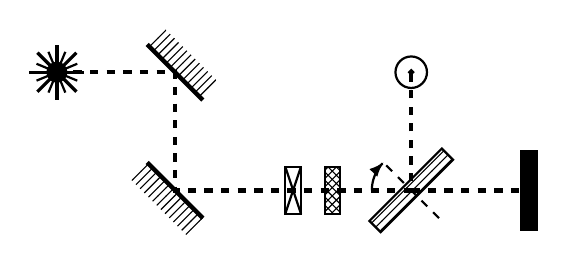
\begin{tikzpicture}
    \coordinate (L) at (0,0);
    \coordinate (M1) at (1.5,0);
    \coordinate (M2) at (1.5,-1.5);
    \coordinate (P1) at (3,-1.5);
    \coordinate (O) at (4.5,-1.5);
    \coordinate (W) at (3.5,-1.5);
    \coordinate (D) at (4.5,0);
    \coordinate (B) at (6,-1.5);

    \def\angle{45};

    % Laser Symbol
    \begin{scope}[scale=0.7]
        \draw[ultra thick, fill = black] (0,0) circle (0.15);
        \draw[rotate=0, very thick] (-0.5,0) -- (0.5,0);
        \draw[rotate=90, very thick] (-0.5,0) -- (0.5,0);
        \draw[rotate=45, very thick] (-0.5,0) -- (0.5,0);
        \draw[rotate=135, very thick] (-0.5,0) -- (0.5,0);

        \draw[rotate=22.5, thick] (-0.4,0) -- (0.4,0);
        \draw[rotate=67.5, thick] (-0.4,0) -- (0.4,0);
        \draw[rotate=112.5, thick] (-0.4,0) -- (0.4,0);
        \draw[rotate=157.5, thick] (-0.4,0) -- (0.4,0);
    \end{scope}

    % Mirror #1
    \begin{scope}[shift={(M1)}, rotate=-45]
        \draw[ultra thick] (-0.5,0) -- (0.5,0);
        \fill[pattern=north east lines] (-0.5,0) rectangle (0.5,0.30);
    \end{scope}

    % Mirror #2
    \begin{scope}[shift={(M2)}, rotate=135]
        \draw[ultra thick] (-0.5,0) -- (0.5,0);
        \fill[pattern=north east lines] (-0.5,0) rectangle (0.5,0.30);
    \end{scope}

    % Polarizer #1
    \begin{scope}[shift={(P1)}, scale=0.5]
        \draw[thick] (-0.2,0.6) rectangle (0.2,-0.6);
        \draw[thick] (-0.2,0.6) -- (0.2,-0.6);
        \draw[thick] (0.2,0.6) -- (-0.2,-0.6);
    \end{scope}

    % Window
    \begin{scope}[shift={(O)}, scale=0.5, rotate=-\angle]
        \draw[thick, pattern=north east lines] (-0.2,1.3) rectangle (0.2,-1.3);

        % Arc
        \draw [->, thick,domain=(180+\angle):(180)] plot ({1*cos(\x)}, {1*sin(\x)}); %node[anchor=south]{$\theta$};

        \draw[dashed, thick] (1,0) -- (-1,0);
    \end{scope}

    % Block
    \begin{scope}[shift={(B)}, scale=0.5, rotate=0]
        \draw[thick, fill=black] (-0.2,1) rectangle (0.2,-1);
    \end{scope}


    % Wave Plate
    \begin{scope}[shift={(3.5,-1.5)}, scale=0.5]
        \draw[thick, pattern=crosshatch] (-0.2,0.6) rectangle (0.2,-0.6);
    \end{scope}

    % Detector
    \begin{scope}[shift={(D)}, scale=0.5]
        \draw[thick] (0,0) circle (0.4);
        \draw[thick, fill=black] (0,0) circle (0.05);
    \end{scope}

    % Beam Path
    \draw[ultra thick, dashed] (L) -- (M1) -- (M2) -- (P1)-- (W) -- (O) -- (D);
    \draw[ultra thick, dashed] (O) -- (B);

\end{tikzpicture}
                \caption{Proposed Experimental Setup for Experiment 3}
                \label{fig:exp3-setup}
            \end{figure}

            The proposed experimental procedure would have been similar to the previous two experiments. However, instead of varying the angle of the polarizer, instead, the dielectric would have been rotated through $180^\circ$ in increments of $10^\circ$. The resultant voltage output would have been recorded for each angle.


    \section{Results \& Analysis}
        \subsection{Polarizers}
            \begin{figure}[H]
                \centering
                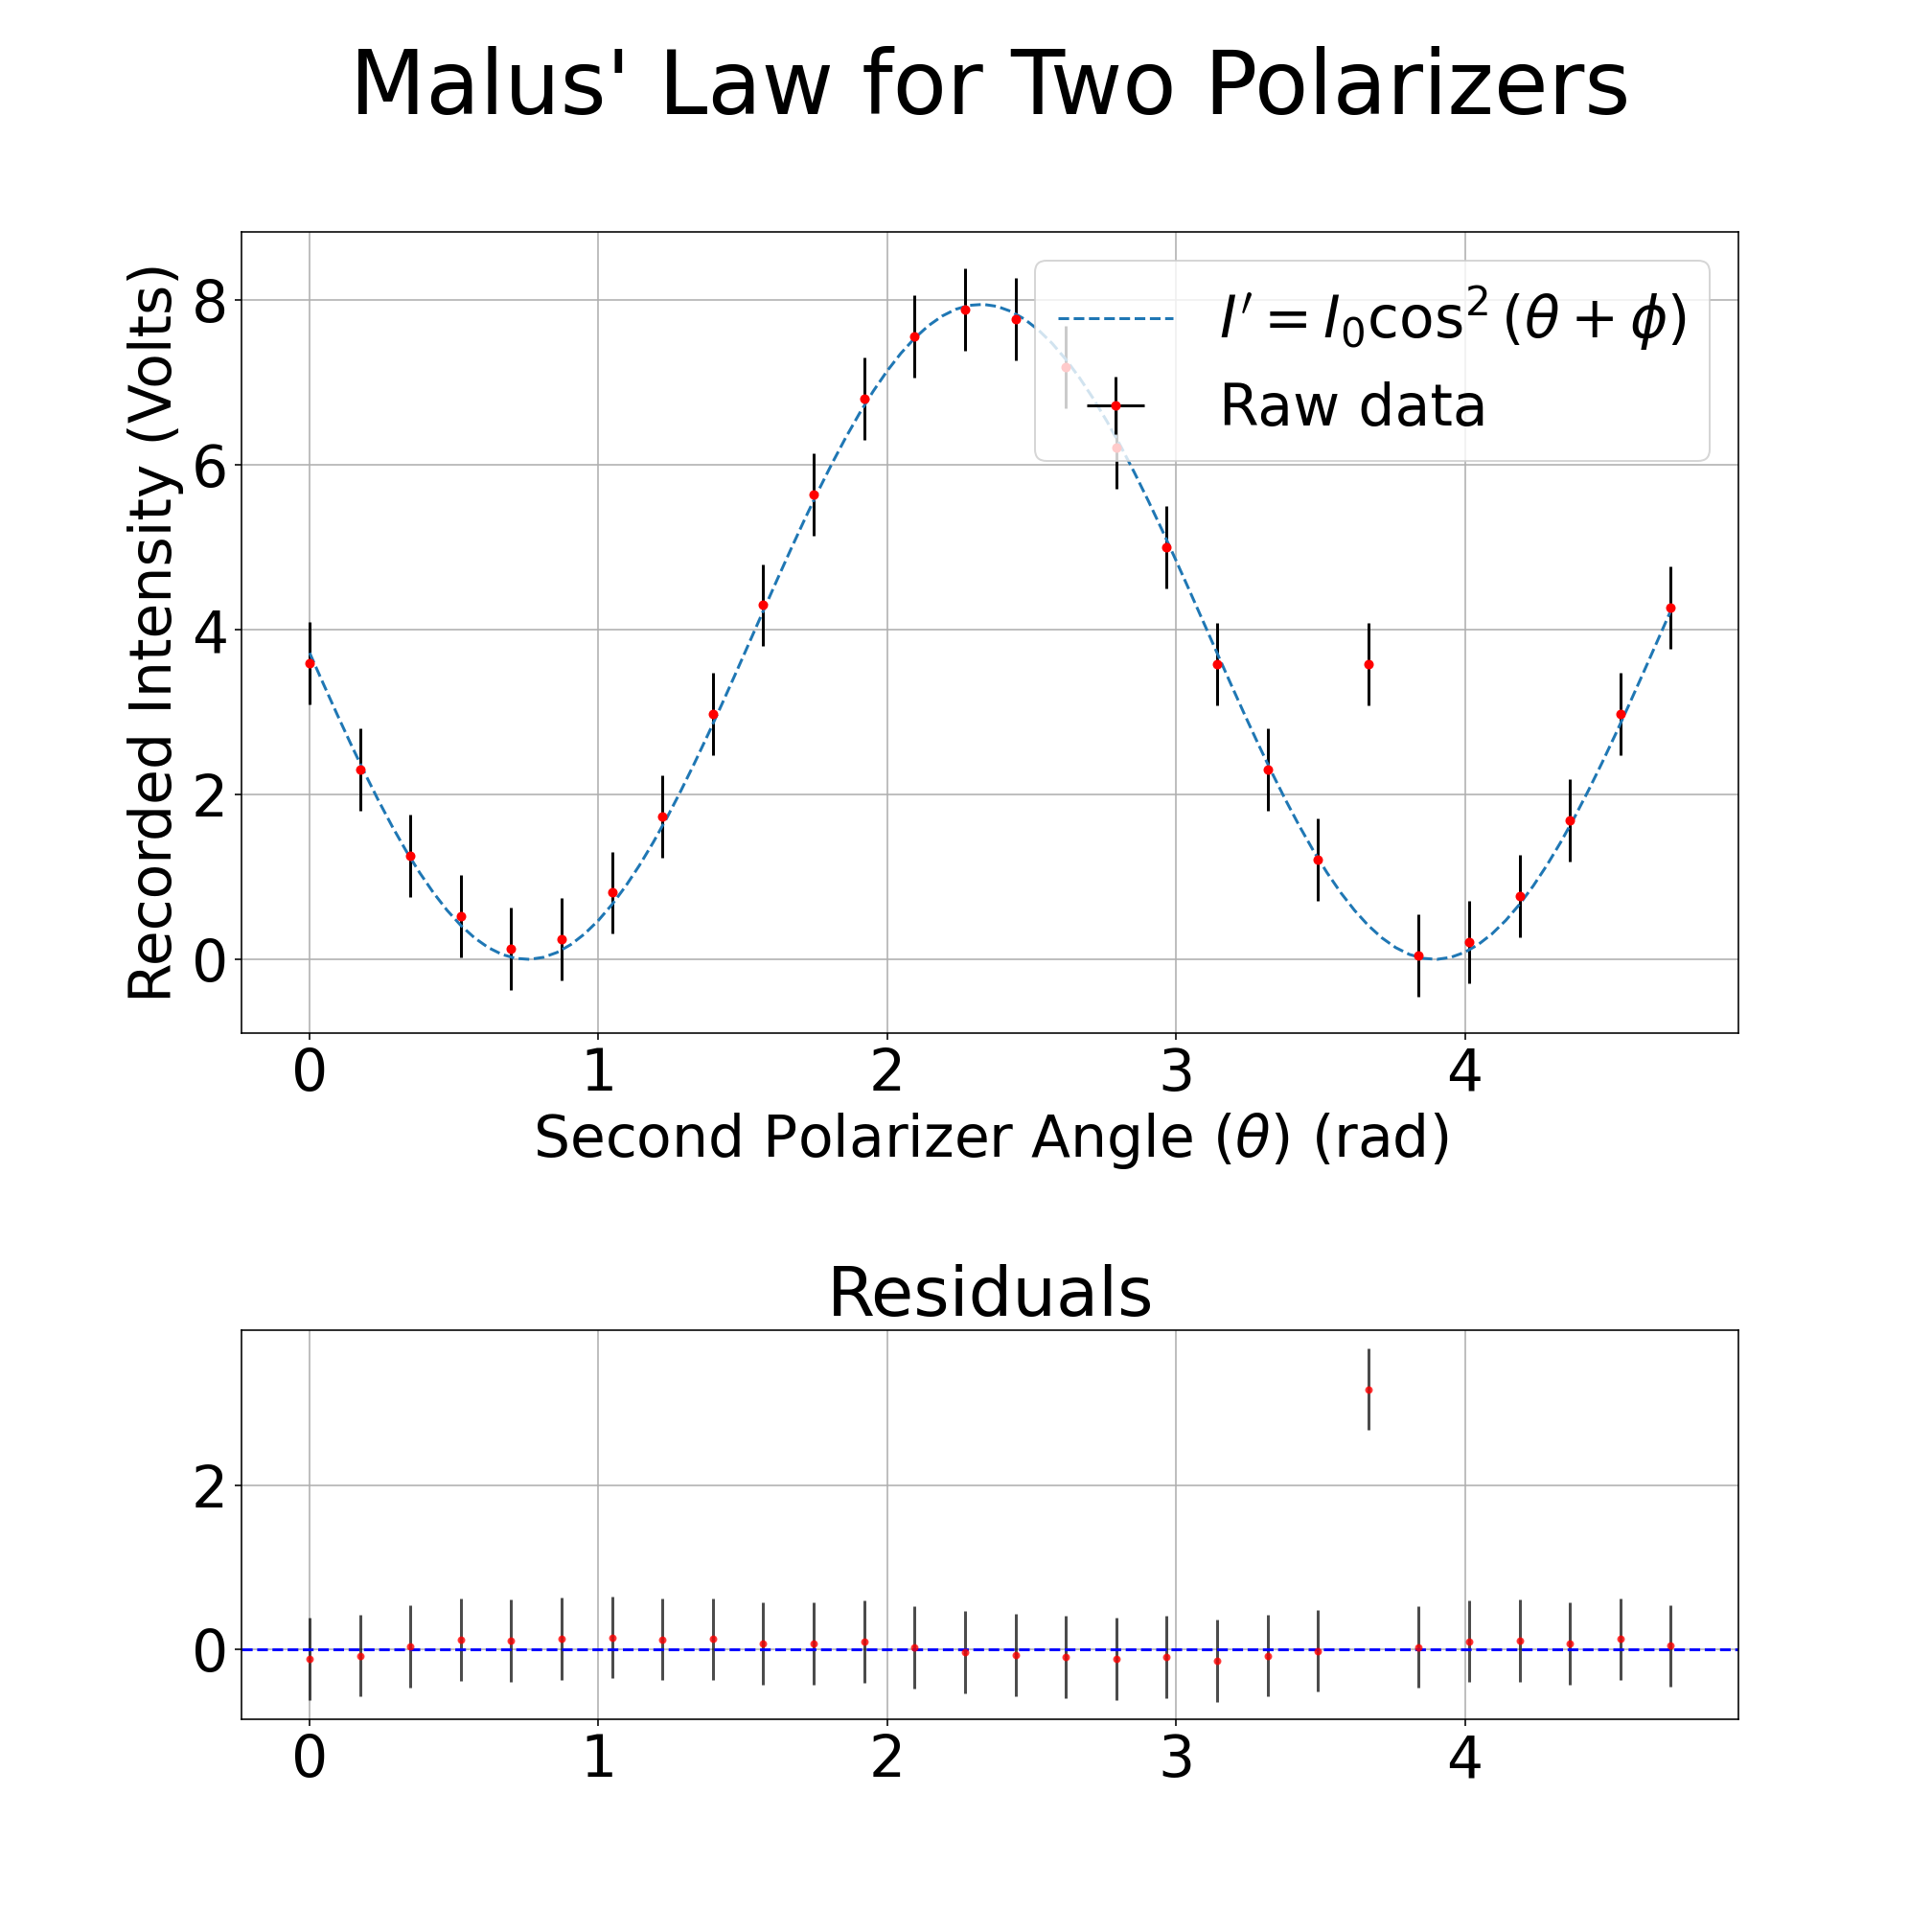
\includegraphics[width=0.9\linewidth]{../figures/Malus.png}
                \caption{Voltage Output vs. Polarizer Angle. $\chi_{red}^2 = 1.58$, $I_0 = 8.0 \pm 0.2\,\text{V}$, $\phi = 0.82 \pm 0.02$}
                \label{fig:part1}
            \end{figure}

            It can clearly be seen in \figref{fig:part1} that the data adheres well to theory. All of the data points, apart from one outlier, falls well within the estimated uncertainty of the fitted curve given in \eqref{eqn:malus}. It should be stated that the $\chi^2$ value of 1.58 is slightly high, however, the lack of a distinct pattern in the residuals indicate that this is a good fit regardless.

            \begin{table}[H]
                \centering
                \begin{tabular}{c|c|c}
                    \bfseries Parameter & \bfseries Value & \bfseries Uncertainty \\
                    \hline
                    $I_0$ & $8.0$ & $0.2$ \\
                    $\phi$ & $0.82$ & $0.02$ \\
                \end{tabular}
            \end{table}

         \subsection{Quarter Waveplate}
            \begin{figure}[H]
                \centering
                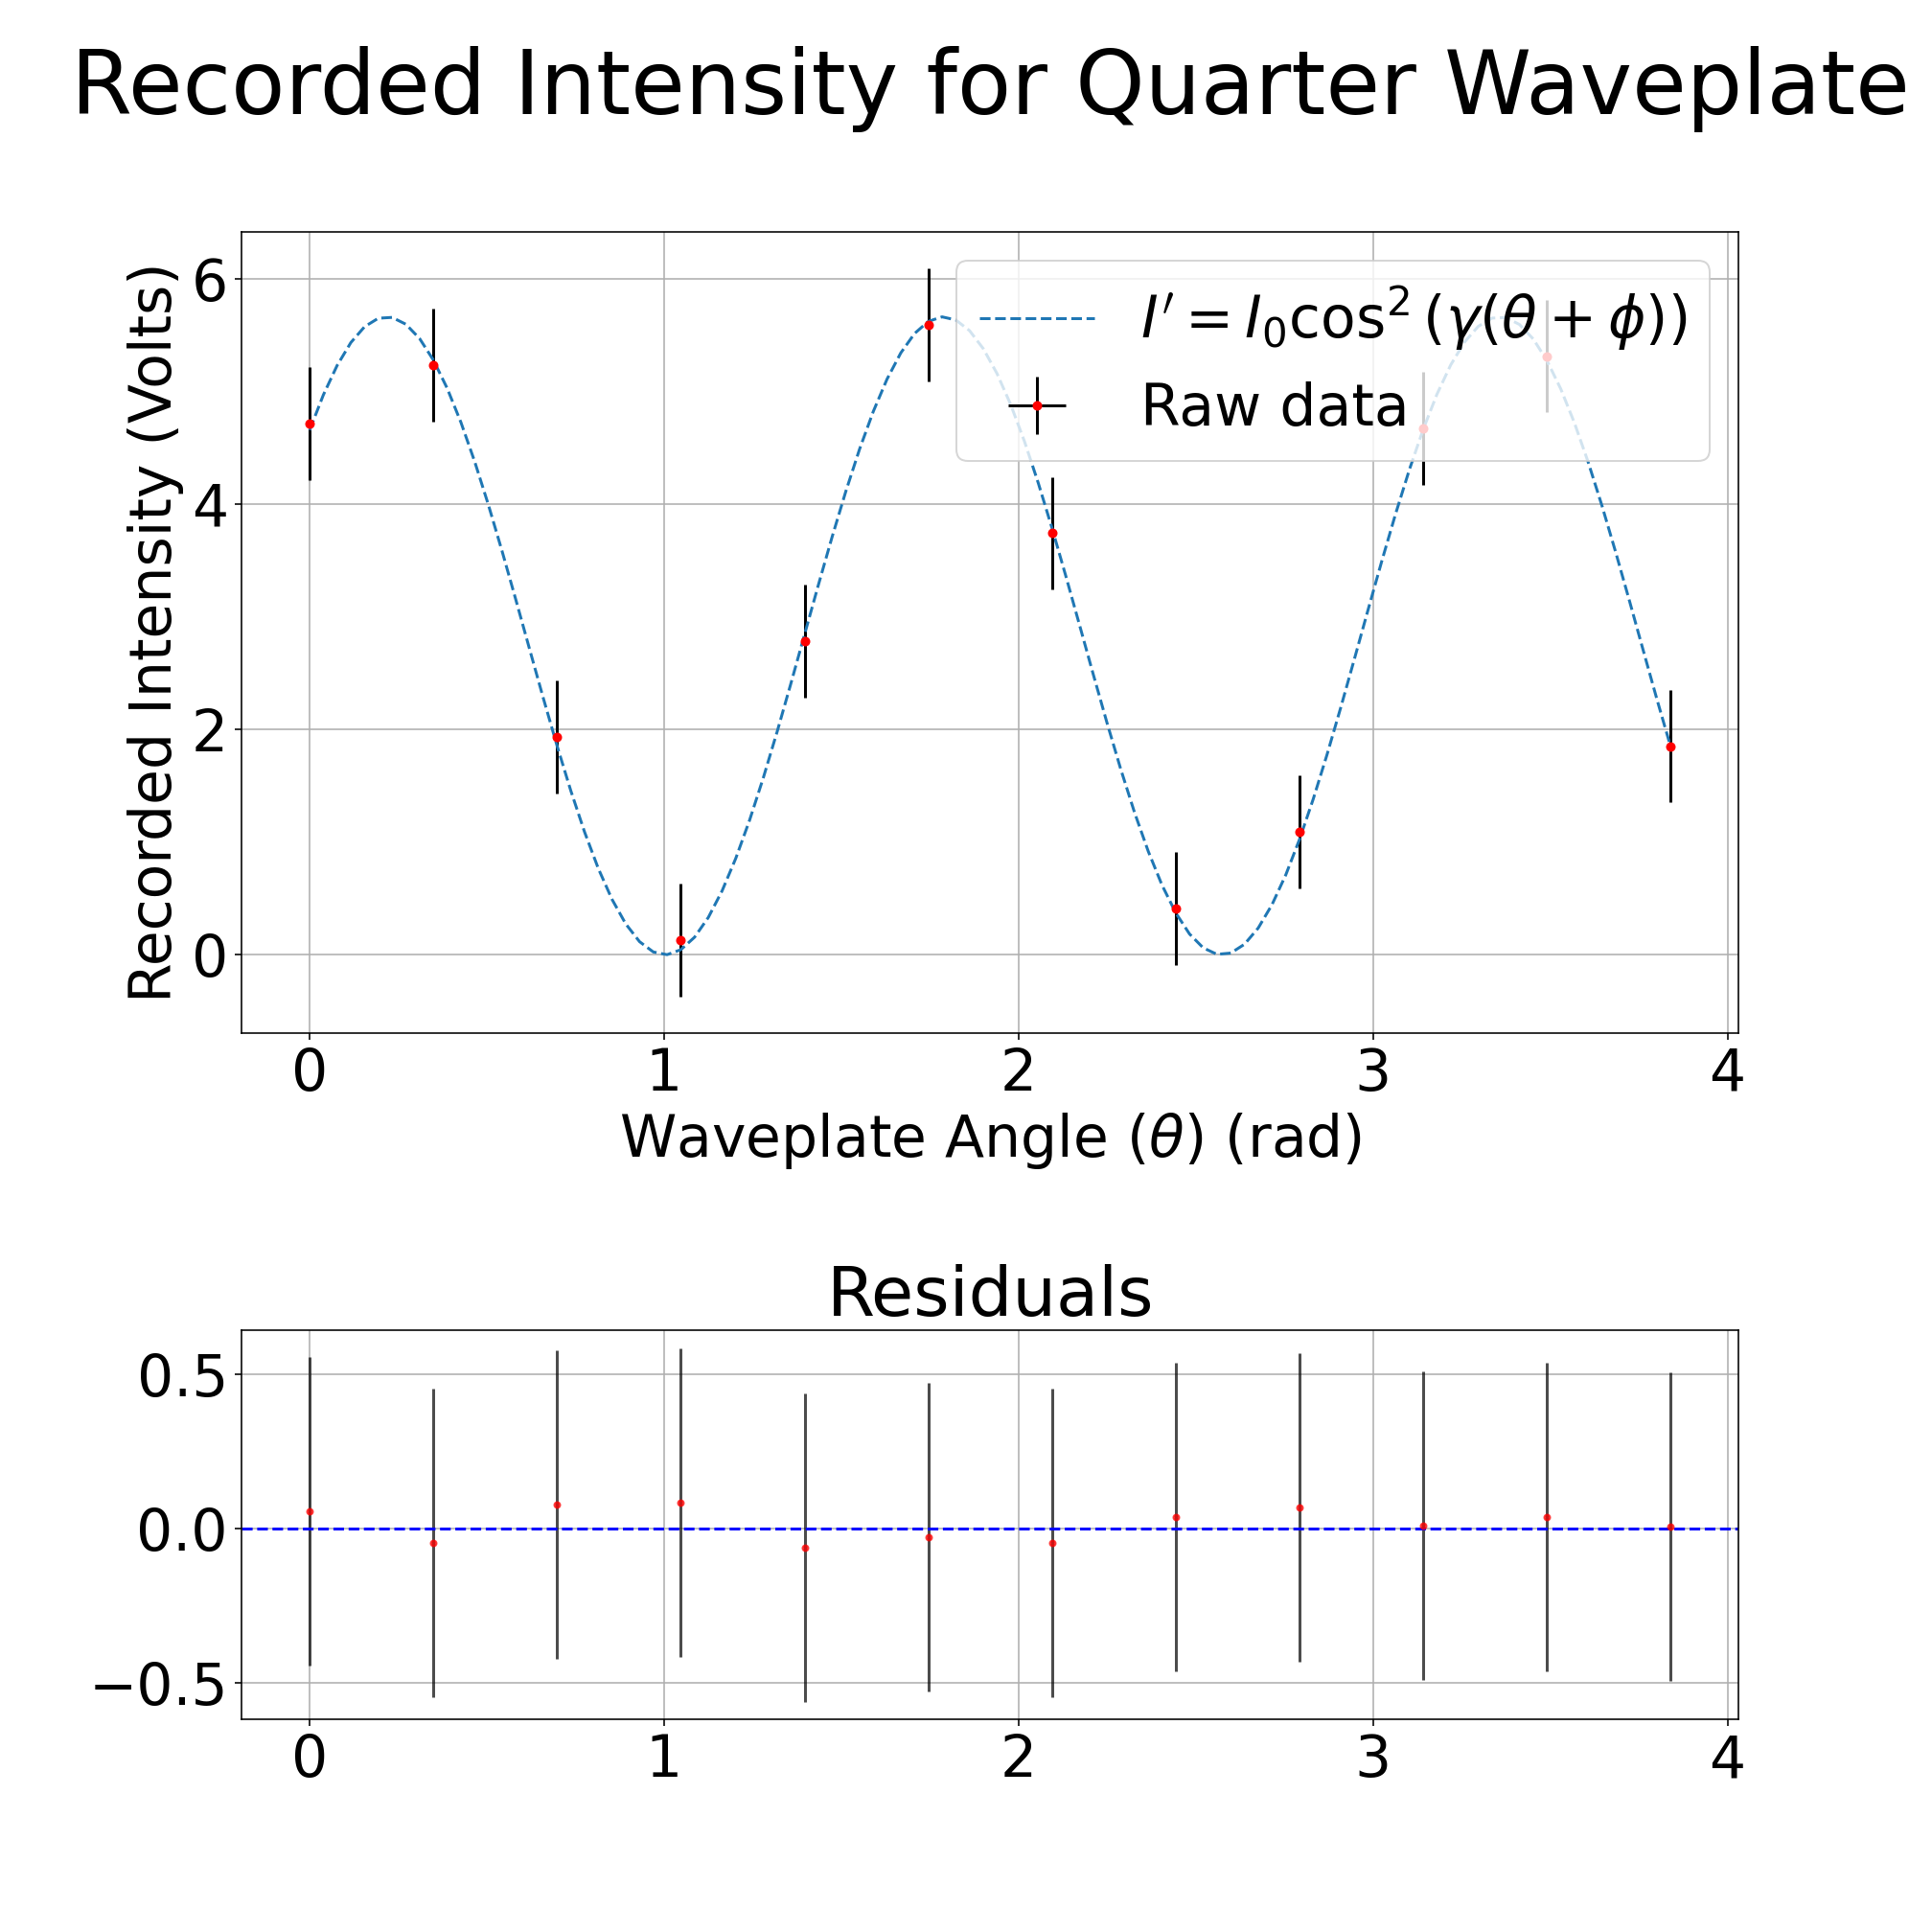
\includegraphics[width=0.9\linewidth]{../figures/Quarter.png}
                \caption{Voltage Output vs. Quarter Waveplate Angle. $\chi_{red}^2 = 0.01$, $I_0 = 5.66 \pm 0.03\,\text{V}$, $\phi = -0.218 \pm 0.004$, $\gamma = 2.001 \pm 0.003$}
                \label{fig:part2a}
            \end{figure}


            In \figref{fig:part2a}, the data adheres well to the theoretical curve. The $\chi^2$ value of 0.01 indicates that the data is a very good fit to the theoretical curve. The residuals are also randomly distributed around zero, indicating that the fit is good.


            \begin{table}[H]
                \centering
                \begin{tabular}{c|c|c}
                    \bfseries Parameter & \bfseries Value & \bfseries Uncertainty \\
                    \hline
                    $I_0$ & $5.66$ & $0.03$ \\
                    $\phi$ & $-0.2175$ & $0.004$ \\
                    $\gamma$ & $2.001$ & $0.003$ \\
                \end{tabular}
            \end{table}

        \subsection{Half Waveplate}
            \begin{figure}[H]
                \centering
                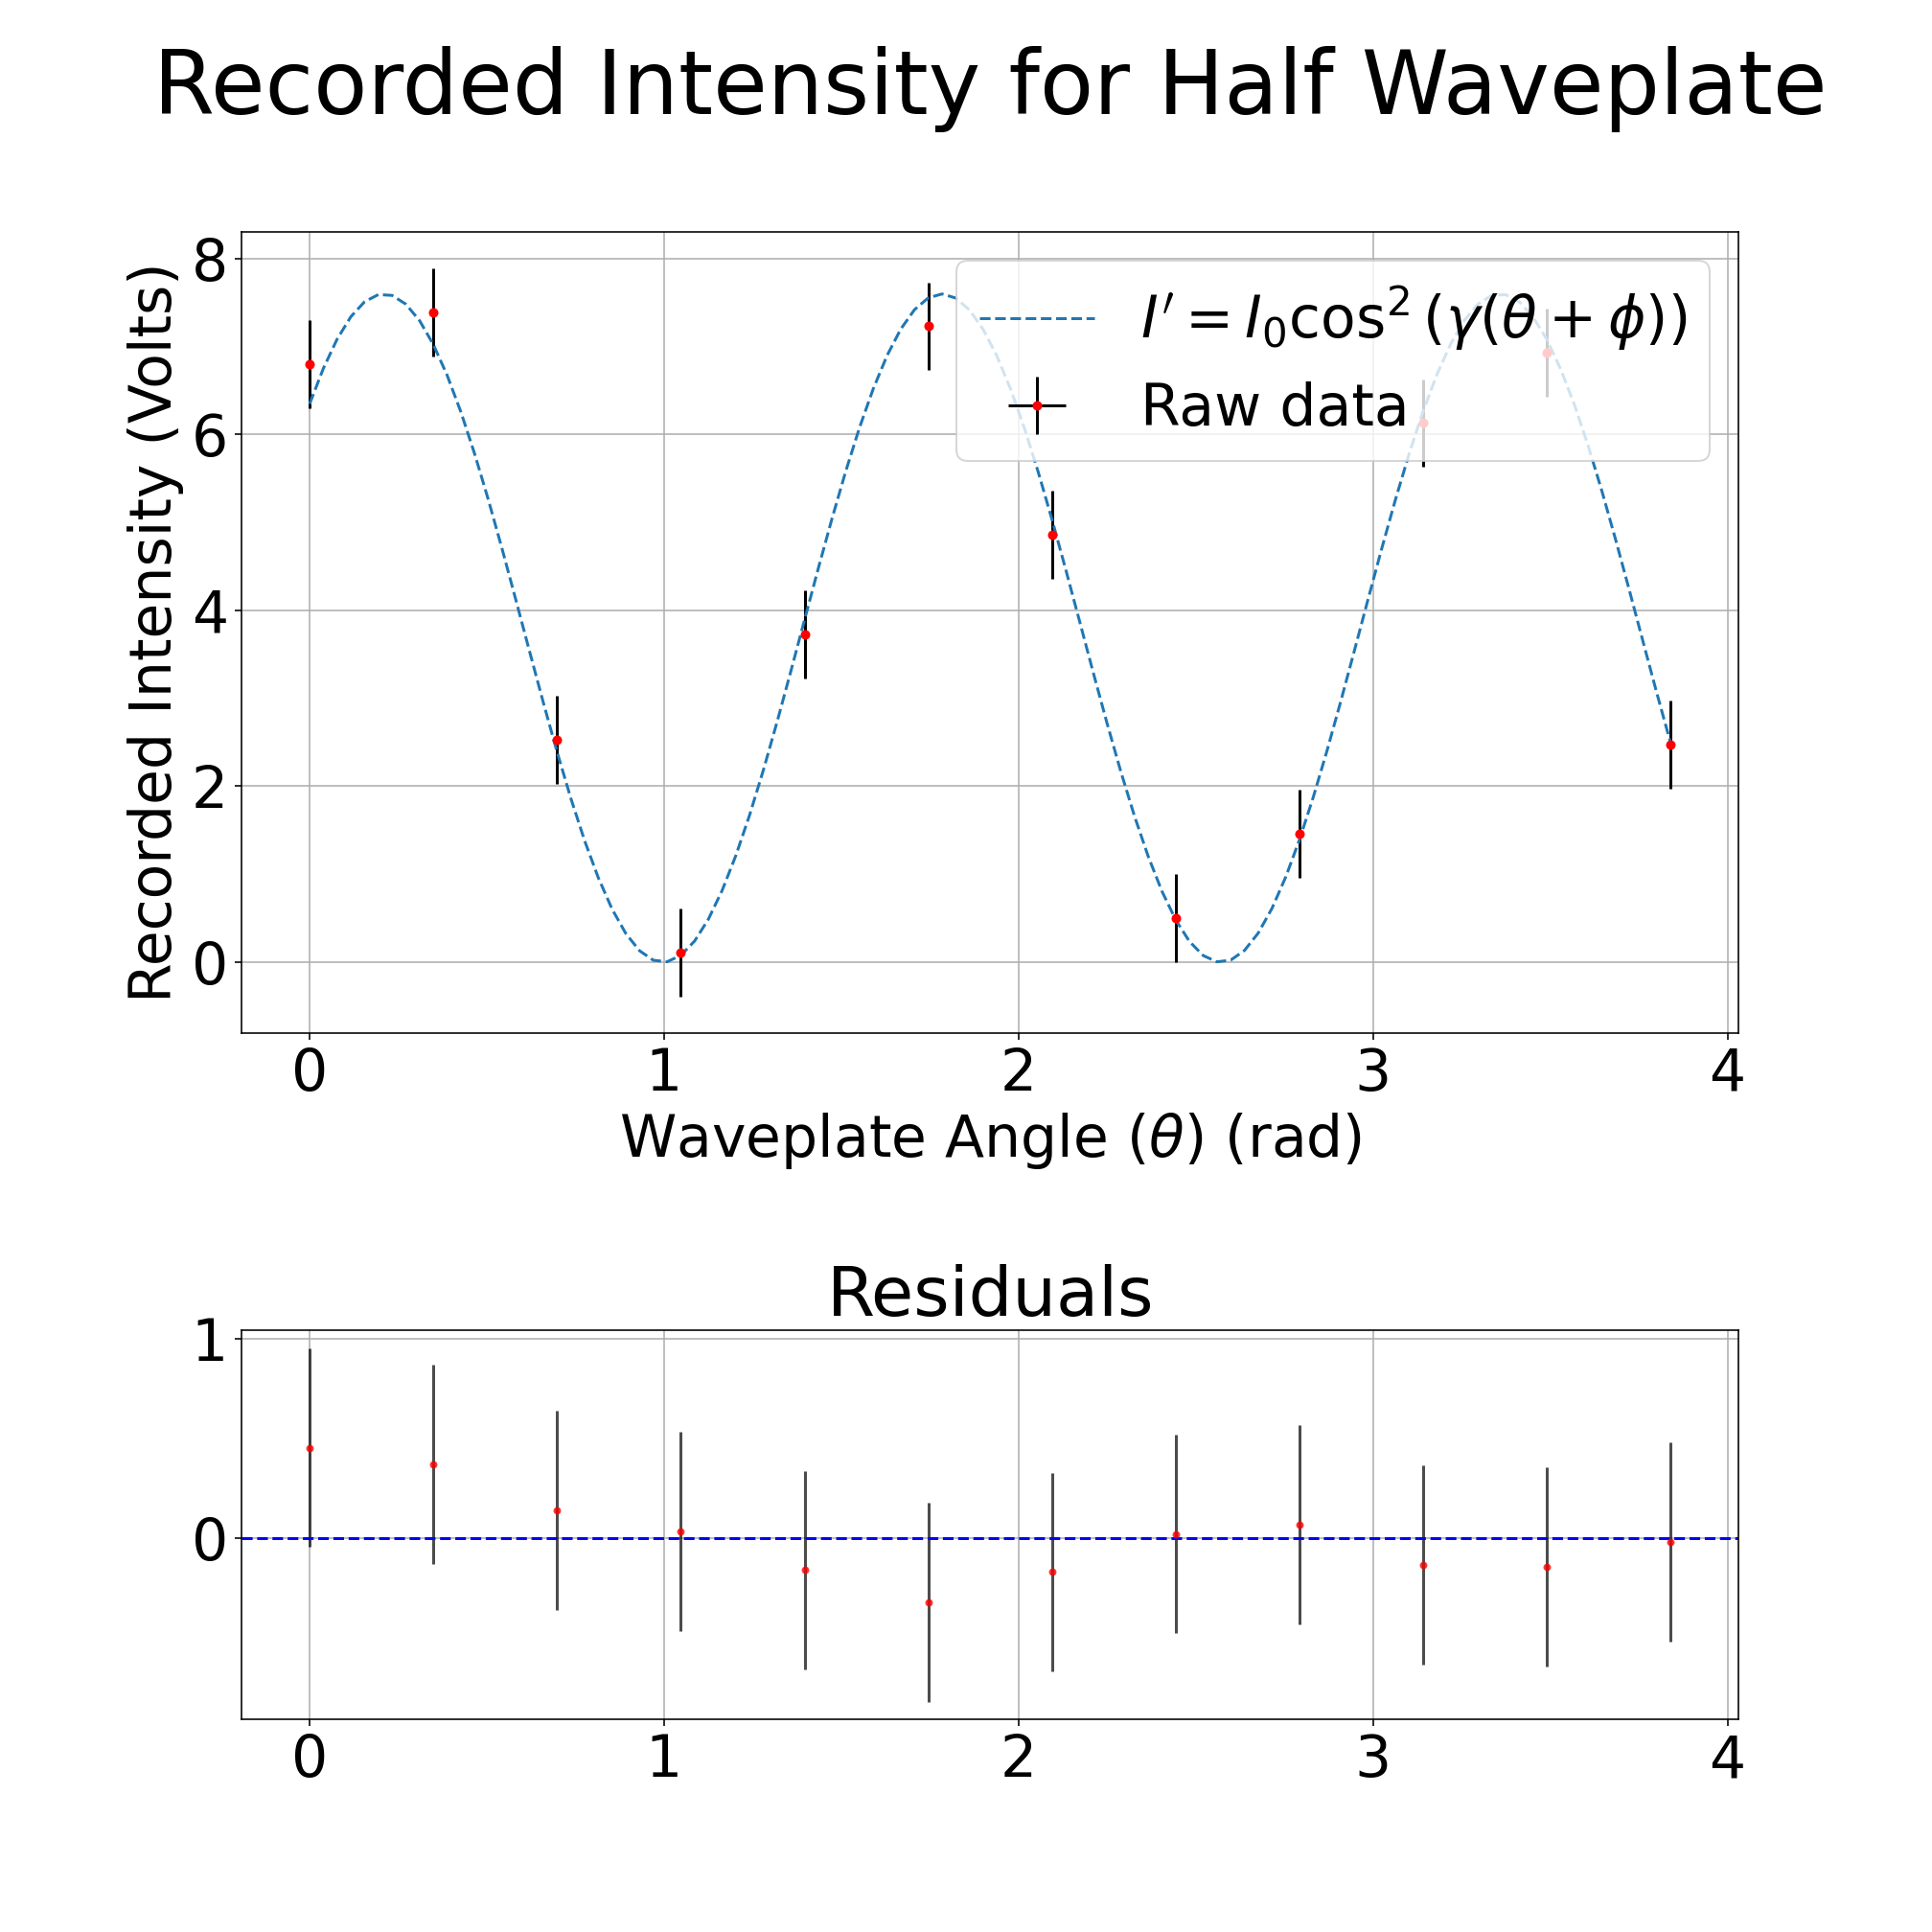
\includegraphics[width=0.9\linewidth]{../figures/Half.png}
                \caption{Voltage Output vs. Half Waveplate Angle. $\chi_{red}^2 = 0.25$, $I_0 = 7.6 \pm 0.1\,\text{V}$, $\phi = -0.21 \pm 0.01$, $\gamma = 2.00 \pm 0.01$}
                \label{fig:part2b}
            \end{figure}


            \begin{table}[H]
                \centering
                \begin{tabular}{c|c|c}
                    \bfseries Parameter & \bfseries Value & \bfseries Uncertainty \\
                    \hline
                    $I_0$ & $7.6$ & $0.1$ \\
                    $\phi$ & $-0.21$ & $0.01$ \\
                    $\gamma$ & $2.00$ & $0.01$ \\
                \end{tabular}
            \end{table}

    
    \section{Discussion}
        An interesting result can be observed in comparing \figref{fig:part2b} and \figref{fig:part1}. The recorded maximum intensity $I_0$ is almost (bar a factor $V = 0.4\,\text{V}$) identical despite the polarizers being set at angles to pass the minimum amount of light. This implies that at $\theta = \frac{\pi}{2}$, the half waveplate effectively makes the second polarizer transparent.

    \section{Conclusion}



    % Line to seperate report content from acknowledgements and references
    \onecolumngrid
    \begin{center}
        \vspace{0.8cm}
        \noindent\rule{0.9\textwidth}{0.5pt}
    \end{center}

    \begin{acknowledgments}
        The work conducted by the other lab partners was instrumental in this lab. Thank you to Jack and Billy for their help in setting up the equipment and conducting the experiments. Additionally, thank you to the Teaching Assistant \taname and Professor \advname for their guidance and support.
    \end{acknowledgments}

\bibliography{references}

\appendix
\section{Appendix}
\subsection{Raw Data}
\subsubsection{Experiment 1: Polarizers}
\begin{table}[H]
    \centering
    \begin{tabular}{l|c|c}%
    \bfseries Polarizer \#1 ($\phantom{\ \ }^{\circ}$) & \bfseries Polarizer \#2 ($\phantom{\ \ }^{\circ}$) & \bfseries Voltage (V)
    \csvreader[head to column names]{../part1.csv}{}% use head of csv as column names
    {\\\hline\Pa &\Pb & \W}% specify your coloumns here
    \end{tabular}
\end{table}

% \subsubsection{Experiment 2: Waveplates}
\subsubsection{Experiment 2: Quarter Waveplate}
\begin{table}[H]
    \centering
    \begin{tabular}{l|c|c|c}%
    \bfseries Polarizer \#1 ($\phantom{\ \ }^{\circ}$) & \bfseries Polarizer \#2 ($\phantom{\ \ }^{\circ}$) & \bfseries QWP ($\phantom{\ \ }^{\circ}$) & \bfseries Voltage (V)
    \csvreader[head to column names]{../part2a.csv}{}% use head of csv as column names
    {\\\hline\Pa &\Pb & \QWP & \W}% specify your coloumns here
    \end{tabular}
\end{table}

%\lstinputlisting{code/part2a.py}

\subsubsection{Experiment 2: Half Waveplate}
\begin{table}[H]
    \centering
    \begin{tabular}{l|c|c|c}%
    \bfseries Polarizer \#1 ($\phantom{\ \ }^{\circ}$) & \bfseries Polarizer \#2 ($\phantom{\ \ }^{\circ}$) & \bfseries HWP ($\phantom{\ \ }^{\circ}$) & \bfseries Voltage (V)
    \csvreader[head to column names]{../part2b.csv}{}% use head of csv as column names
    {\\\hline\Pa &\Pb & \HWP & \W}
    \end{tabular}
\end{table}


\subsection{Analysis Code}
\subsubsection{Experiment 1: Polarizers}
\lstinputlisting{../part1.py}
\subsubsection{Experiment 2: Waveplates}
\lstinputlisting{../part2.py}
\subsubsection{Toolkit}
\lstinputlisting{../toolkit.py}

\end{document}\subsubsection{Experiment 2: Waveplates}